\chapter{Project management}

\section{Project plan}
\subsection{Tool Selection}

\subsection{Concrete Project Work Plan}

\begin{figure}
\centering
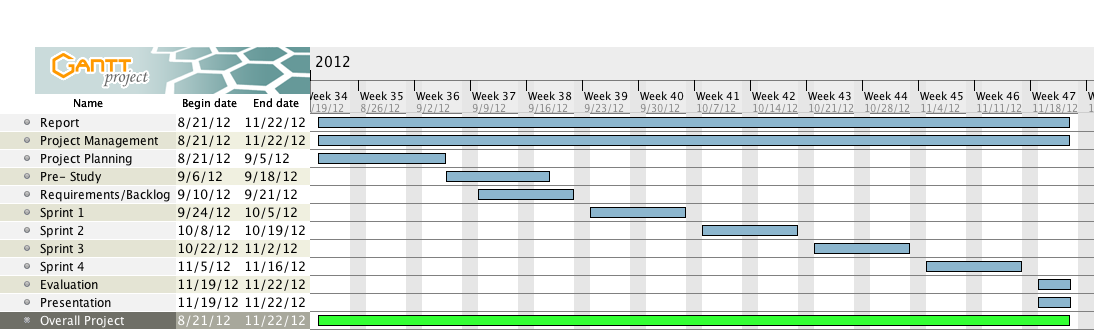
\includegraphics[width=6in]{image/gantt.png}
\caption{Gantt Chart}
\label{figure:gantt}
\end{figure}

\begin{table}
\caption{Work Breakdown Structure}
\centering
\begin{tabular}{ l l l l l }
\hline 
			&				&				&\multicolumn{2}{c}{Hours}		\\
 Task		& From date		&To date			&Est.			&Act.	                \\ 
\hline \\ [-2.0ex]
 The report     			&21/08/2012		&22/11/2012		&300		&         	 \\
 Project Management	&21/08/2012		&22/11/2012		&180		&		\\
 Project Planning		&21/08/2012		&05/09/2012		&100		&		\\
 Lectures				&21/08/2012		&05/09/2012		&40			&		\\	
 Pre- Study			&06/09/2012		&18/09/2012		&80			&		\\
 Backlog				&10/09/2012		&21/09/2012		&60			&		\\
 Architecture			&17/09/2012		&21/09/2012		&40			&		\\
\hline \\ [-2.0ex]
 \bf{Sprint 1}			&\bf{24/09/2012}	&\bf{05/10/2012}	&\bf{130}		&		\\
 Planning				&				&				&20			&		\\
 Design/Implementation	&				&				&90			&		\\
 Testing				&				&				&20			&		\\
\hline \\ [-2.0ex]
 \bf{Sprint 2}			&\bf{08/10/2012}	&\bf{19/10/2012}	&\bf{130}		&		\\
 Planning				&				&				&20			&		\\
 Design/Implementation	&				&				&90			&		\\
 Testing				&				&				&20			&		\\
\hline \\ [-2.0ex]
 \bf{Sprint 3}			&\bf{22/10/2012}	&\bf{02/11/2012}	&\bf{140}		&		\\
 Planning				&				&				&20			&		\\
 Design/Implementation	&				&				&100		&		\\
 Testing				&				&				&20			&		\\
\hline \\ [-2.0ex]
 \bf{Sprint 4}			&\bf{05/11/2012}	&\bf{16/11/2012}	&\bf{140}		&		\\
 Planning				&				&				&20			&		\\
 Design/Implementation	&				&				&100		&		\\
 Testing				&				&				&20			&		\\
\hline \\ [-2.0ex]
 Evaluation			&19/11/2012		&22/11/2012		&30			&		\\
 Presenation			&19/11/2012		&21/11/2012		&30			&		\\
\hline \\ [-2.0ex]
 \bf{Total}			&				&				&\bf{1400}	&		\\
\hline
\end{tabular}
\label{table:wbs}
\end{table}

\section{Project name}
Project name is important project identificator. It should summarize main project goal or functionality. In real project, is often a trademark, or reflects the name of the company.

In this section, we will describe the process of choosing a name for the project. First of all, we made a list of words, that we can use in the project name. These words describe project funcionality or goal.

Words that can be used in project name: master, console, web, text, keyboard

We used the list of words and brainstorming session on a meeting for compiling a list of project name candidates:

Candidate project names: console 2.0, wonsole, wensole, websole, werminal, interCLI

After discussion we chose the name \emph{Wonsole}. Project name can be sometimes little confusing, so we added the subtitle: \emph{The new web console for power users.}


\section{Team Structure}

\subsection{Team Roles}
\begin{table}
\begin{tabularx}{\textwidth}{ | l | X | l | }
  \hline
  \textbf{Team member} & \textbf{Roles} \\ \hline
  Ivo & Group leader, Customer and Advisor Contact, Scrum Master \\ \hline
  Oystein & Test Manager, QA Manager, Weekly Report Manager \\ \hline
  Oddvar & GUI Designer, Code Master, Meeting Secretary, Time Keeper \\ \hline
  Martin & System Architect, Report Manager \\ \hline
\end{tabularx}
\caption{Team role overview}
\end{table}



\begin{table}
\begin{tabularx}{\textwidth}{ | l | X | l | }
  \hline
  \textbf{Role} & \textbf{Description} & \textbf{Assignee} \\ 
  \hline
  Team leader & Is responsible for administrative tasks and makes the final decisions. & Ivo \\ 
  \hline
  Scrum Master & Shields the development team from external distractions and enforces the Scrum scheme.  & Ivo \\ 
  \hline
  Customer Contact & Handles communication with the customer. The customer should contact this person regarding general requests, questions and reminders. & Ivo (backup Martin) \\ 
  \hline
  Advisor Contact & Handles communication with the advisor. The advisor should contact this person regarding general requests, questions and reminders.  & Ivo (backup Martin) \\ 
  \hline
  System Architect & Is responsible for the system architecture including distinctions and relations between subsystems and general code design choices. & Martin \\ 
  \hline
  Code Master & Overall responsible for code management and structure. Managing branches in Git repository. & Oddvar  \\ 
  \hline
  GUI Designer & Is responsible for the layout and design of graphical user interfaces. & Oddvar \\ 
  \hline
  Test Manager & Is responsible for testing including unit tests, integration tests and usability tests. & Øystein \\ 
  \hline
  Report Manager & Is responsible for delegating and overseeing work on the project report. & Martin \\ 
  \hline
  Customer Representative & Participates in regular meetings to discuss the progress, project status and future tasks. Represents the customer. & Peder Kongelf \\ 
  \hline
  Customer Technical Advisor & May be consulted about technical aspects of the project. & Stig Lau \\ 
  \hline
  Advisor & Serves as a one-man steering committee for the project. & Meng Zhu \\ 
  \hline
  Meeting Secretary & Is responsible for making sure notes get written and sent after each meeting with the advisor and customer. & Oddvar \\ 
  \hline
  Quality Assurance Manager &  & Øystein \\ 
  \hline
  Weekly Report Writer & Is responsible for finalizing the weekly report(s) for the advisor and customer, and getting these delivered for approval. Also responsible for meeting agendas and their delivery. & Øystein \\ 
  \hline
  Time Keeper & Responsible for making sure that everybody is logging their work, and logging team activities. & Oddvar \\ 
  \hline
\end{tabularx}
\caption{Team role}
\end{table}

\section{Quality Assurance}
\subsection{Communication rules}
To prevent misunderstanding in communication and

\begin{table}
\begin{tabularx}{\textwidth}{ | c | X | }
  \hline
  meeting & scheduled at least 48 hours before, confirmation within 24 hours before meeting required \\ \hline
  documents for the meeting & 24 hours before \\ \hline
  email communication & contact person directly, google groups is just internal \\ \hline
  response from the team & within 8 hours \\ \hline
  response from customer & within 24 hours \\ \hline
\end{tabularx}
\caption{Communication rules}
\end{table}

\section{Risks}
\chapter{Risk Table}

\begin{table}
\begin{tabularx}{\textwidth}{ | l | X | l | l | }
  \hline
  \textbf{\#} & \textbf{Risk} & \textbf{Probability} & \textbf{Impact} \\ \hline
  1 & Not getting a fifth party member & M & Significant \\ \hline
  2 & Obtrusive health/family/personal issues for team members & L & Significant \\ \hline
  3 & Low morale in team & M & Significant \\ \hline
  4 & Interfering workload from other activities & H & Minor \\ \hline
  5 & Miscommunication with customer & M & Critical \\ \hline
  6 & Changes in customer requirements & M & Significant \\ \hline
  7 & Errors in project plan & M & Significant \\ \hline
  8 & Failure of communication in team & M & Critical \\ \hline
  9 & Failure of time management & H & Critical \\ \hline
 10 & Errors in workload estimation and distribution & H & Critical \\ \hline
 11 & Failure of online storage systems and services & L & Significant \\ \hline
 12 & Failure of personal computers & M & Significant \\ \hline
 13 & Infeasibility of project as a whole & L & Critical \\ \hline
 14 & Inability to find potential users and test subjects & M & Significant \\ \hline
\end{tabularx}
\caption{Risk overview}
\end{table}


\begin{table}
\begin{tabularx}{\textwidth}{ | l | X | }
\hline
\textbf{Risk \#} & 01 \\ \hline
\textbf{Activity} & All \\ \hline
\textbf{Risk Factor} & Not getting a fifth party member \\ \hline
\textbf{Impact} & Significant \\ \hline
\textbf{Consequence} & Increased workload for all remaining party members on all activities \\ \hline
\textbf{Probability} & Medium \\ \hline
\textbf{Countermeasures} & \begin{itemize}
  \item  Contact advisor about the dropped party member, try to get assigned a new member.
  \item Take the missing person into account in planning phase.
\end{itemize}  \\ \hline
\textbf{Deadline} & Intro/Planning (Ultimately in the hands of course staff) \\ \hline
\textbf{Responsible} & Project leader \\ \hline
\end{tabularx}
\caption{Risk 01}
\end{table}

\medskip

\begin{table}
\begin{tabularx}{\textwidth}{ | l | X | }
\hline
\textbf{Risk \#} & 02 \\ \hline
\textbf{Activity} & All \\ \hline
\textbf{Risk Factor} & Obtrusive health/family/personal issues for team members \\ \hline
\textbf{Impact} & Significant \\ \hline
\textbf{Consequence} & Increased workload for all remaining party members on all activities \\ \hline
\textbf{Probability} & Low  \\ \hline
\textbf{Countermeasures} & \begin{itemize}
  \item Implement buffers in project plan.
  \item Team members should make their work resumable by another member.
\end{itemize}  \\ \hline
\textbf{Deadline} &  None \\ \hline
\textbf{Responsible} & Project leader \\ \hline
\end{tabularx}
\caption{Risk 02}
\end{table}

\medskip

\begin{table}
\begin{tabularx}{\textwidth}{ | l | X | }
\hline
\textbf{Risk \#} & 03 \\ \hline
\textbf{Activity} & All \\ \hline
\textbf{Risk Factor} & Low morale in team \\ \hline
\textbf{Impact} & Significant \\ \hline
\textbf{Consequence} & Decreased overall project quality \\ \hline
\textbf{Probability} & Medium  \\ \hline
\textbf{Countermeasures} & \begin{itemize}
  \item Frequent contact between team members
  \item Avoid team members overworking
  \item Focus on general team dynamics advice from advisor
\end{itemize}  \\ \hline
\textbf{Deadline} &  None \\ \hline
\textbf{Responsible} & Project leader \\ \hline
\end{tabularx}
\caption{Risk 03}
\end{table}

\medskip

\begin{table}
\begin{tabularx}{\textwidth}{ | l | X | }
\hline
\textbf{Risk \#} & 04 \\ \hline
\textbf{Activity} & All \\ \hline
\textbf{Risk Factor} & Interfering workload from other activities \\ \hline
\textbf{Impact} & Low \\ \hline
\textbf{Consequence} & Work on the project is shifted in time, space and responsibility \\ \hline
\textbf{Probability} & Very High \\ \hline
\textbf{Countermeasures} & \begin{itemize}
  \item Plan ahead with respect to existing schedules
  \item Inform the group of other activities
\end{itemize}  \\ \hline
\textbf{Deadline} &  None \\ \hline
\textbf{Responsible} & Project leader \\ \hline
\end{tabularx}
\caption{Risk 04}
\end{table}

\medskip

\begin{table}
\begin{tabularx}{\textwidth}{ | l | X | }
\hline
\textbf{Risk \#} & 05 \\ \hline
\textbf{Activity} & All \\ \hline
\textbf{Risk Factor} & Miscommunication with customer \\ \hline
\textbf{Impact} & Critical \\ \hline

\textbf{Consequence} & -The project is not developed as the customer wants it
-Work has to be done over \\ \hline
\textbf{Probability} & Very High \\ \hline
\textbf{Countermeasures} & \begin{itemize}
  \item Weekly customer meetings
  \item Share as much information as possible with customer at all stages
\end{itemize}  \\ \hline
\textbf{Deadline} &  None \\ \hline
\textbf{Responsible} & Customer Contact \\ \hline
\end{tabularx}
\caption{Risk 05}
\end{table}

\medskip

\begin{table}
\begin{tabularx}{\textwidth}{ | l | X | }
\hline
\textbf{Risk \#} & 06 \\ \hline
\textbf{Activity} & Planning, Requirements, Implementation \\ \hline
\textbf{Risk Factor} & Changes in customer requirements \\ \hline
\textbf{Impact} & Significant \\ \hline
\textbf{Consequence} & Work has to be done over  \\ \hline
\textbf{Probability} & Medium \\ \hline
\textbf{Countermeasures} & \begin{itemize}
  \item Design the prototype with possible modifications in mind.
  \item Try to get information on possible changes from the customer.
\end{itemize}  \\ \hline
\textbf{Deadline} &  None \\ \hline
\textbf{Responsible} & Customer Contact \\ \hline
\end{tabularx}
\caption{Risk 06}
\end{table}

\medskip

\begin{table}
\begin{tabularx}{\textwidth}{ | l | X | }
\hline
\textbf{Risk \#} & 07 \\ \hline
\textbf{Activity} & Implementation \\ \hline
\textbf{Risk Factor} & Errors in project plan \\ \hline
\textbf{Impact} & Significant \\ \hline
\textbf{Consequence} & Work on the plan and implementation have to be redone  \\ \hline
\textbf{Probability} & Medium \\ \hline
\textbf{Countermeasures} & \begin{itemize}
  \item Review the project plan frequently for consistency
  \item Share plan with customer
\end{itemize}  \\ \hline
\textbf{Deadline} &  Planning \\ \hline
\textbf{Responsible} & Project Leader \\ \hline
\end{tabularx}
\caption{Risk 07}
\end{table}

\medskip

\begin{table}
\begin{tabularx}{\textwidth}{ | l | X | }
\hline
\textbf{Risk \#} & 08 \\ \hline
\textbf{Activity} & All \\ \hline
\textbf{Risk Factor} & Failure of communication in team \\ \hline
\textbf{Impact} & Critical \\ \hline
\textbf{Consequence} & Failure of unification of the work, uneven workloads, decreased project quality  \\ \hline
\textbf{Probability} & Medium \\ \hline
\textbf{Countermeasures} & \begin{itemize}
  \item Frequent internal meetings
  \item Sharing of work internally
\end{itemize}  \\ \hline
\textbf{Deadline} &  None \\ \hline
\textbf{Responsible} & Project Leader \\ \hline
\end{tabularx}
\caption{Risk 08}
\end{table}

\medskip

\begin{table}
\begin{tabularx}{\textwidth}{ | l | X | }
\hline
\textbf{Risk \#} & 09 \\ \hline
\textbf{Activity} & All \\ \hline
\textbf{Risk Factor} & Failure of time management \\ \hline
\textbf{Impact} & Critical \\ \hline
\textbf{Consequence} & Parts of project are rushed or not finished in time \\ \hline
\textbf{Probability} & High \\ \hline
\textbf{Countermeasures} & \begin{itemize}
  \item Put in as much work as possible as early as possible
  \item Implement buffers in project plan
\end{itemize}  \\ \hline
\textbf{Deadline} &  None \\ \hline
\textbf{Responsible} & Project Leader \\ \hline
\end{tabularx}
\caption{Risk 09}
\end{table}

\medskip

\begin{table}
\begin{tabularx}{\textwidth}{ | l | X | }
\hline
\textbf{Risk \#} & 10 \\ \hline
\textbf{Activity} & All \\ \hline
\textbf{Risk Factor} & Errors in workload estimation and distribution \\ \hline
\textbf{Impact} & Critical \\ \hline
\textbf{Consequence} & Uneven workloads, rushed or unfinished parts of project \\ \hline
\textbf{Probability} & High \\ \hline
\textbf{Countermeasures} & \begin{itemize}
  \item Implement buffers in project plan
  \item Avoid relying too much on rigid plans
  \item Allow for redistribution of work when necessary
\end{itemize}  \\ \hline
\textbf{Deadline} &  Planning \\ \hline
\textbf{Responsible} & Project Leader \\ \hline
\end{tabularx}
\caption{Risk 10}
\end{table}

\medskip

\begin{table}
\begin{tabularx}{\textwidth}{ | l | X | }
\hline
\textbf{Risk \#} & 11 \\ \hline
\textbf{Activity} & All \\ \hline
\textbf{Risk Factor} & Failure of online storage systems and services \\ \hline
\textbf{Impact} & Critical \\ \hline
\textbf{Consequence} & Work is lost and has to be recreated \\ \hline
\textbf{Probability} & Low \\ \hline
\textbf{Countermeasures} & \begin{itemize}
  \item Local backups of data
  \item Know of alternative systems in case of failure
\end{itemize}  \\ \hline
\textbf{Deadline} &  None \\ \hline
\textbf{Responsible} & Project Leader \\ \hline
\end{tabularx}
\caption{Risk 11}
\end{table}

\medskip

\begin{table}
\begin{tabularx}{\textwidth}{ | l | X | }
\hline
\textbf{Risk \#} & 12 \\ \hline
\textbf{Activity} & All \\ \hline
\textbf{Risk Factor} & Failure of personal computers \\ \hline
\textbf{Impact} & Significant \\ \hline
\textbf{Consequence} & Work may be lost, decreased productivity of team member \\ \hline
\textbf{Probability} & Medium \\ \hline
\textbf{Countermeasures} & \begin{itemize}
  \item Use primarily online storage systems and keep online backups of everything else
  \item Use university computers if necessary
\end{itemize}  \\ \hline
\textbf{Deadline} &  None \\ \hline
\textbf{Responsible} & Individual \\ \hline
\end{tabularx}
\caption{Risk 12}
\end{table}

\medskip

\begin{table}
\begin{tabularx}{\textwidth}{ | l | X | }
\hline
\textbf{Risk \#} & 13 \\ \hline
\textbf{Activity} & All \\ \hline
\textbf{Risk Factor} & Infeasibility of project as a whole \\ \hline
\textbf{Impact} & Critical \\ \hline
\textbf{Consequence} & The concept is not a solution to the problem and the prototype is destined to be a failure \\ \hline
\textbf{Probability} & Very Low \\ \hline
\textbf{Countermeasures} & \begin{itemize}
  \item Extensive preliminary study to uncover this as early as possible
\end{itemize}  \\ \hline
\textbf{Deadline} & Feasibility study \\ \hline
\textbf{Responsible} & Project Leader \\ \hline
\end{tabularx}
\caption{Risk 13}
\end{table}

\medskip

\begin{table}
\begin{tabularx}{\textwidth}{ | l | X | }
\hline
\textbf{Risk \#} & 14 \\ \hline
\textbf{Activity} & Planning \\ \hline
\textbf{Risk Factor} & Inability to find potential users and test subjects \\ \hline
\textbf{Impact} & Significant \\ \hline
\textbf{Consequence} & Requirements engineering and prototype testing will be sub-standard unable to provide adequate answers \\ \hline
\textbf{Probability} & Medium \\ \hline
\textbf{Countermeasures} & \begin{itemize}
  \item Try to get information on potential users from customer
  \item Begin contacting potential users and testers early
\end{itemize}  \\ \hline
\textbf{Deadline} & Testing \\ \hline
\textbf{Responsible} & Project Leader \\ \hline
\end{tabularx}
\caption{Risk 14}
\end{table}



\section{Meetings}
\section{Lectures}
\section{Issues}
\section{Scrum}


\section{Domain choosing}
\begin{comment}
Domain ideas:
project management tool (ehm. redmine)
warehouse
airport / travel agency
cash registers (not interesting)
bank
school information system (boring)
time management system (aka calendar)
facebook console (unreal)
mail interface (gmail is too good, not useful)
photo gallery (limited)
music library (limited)
physician system (treatments, prescriptions, add person)
tax form (boring)
Building management (boring)
Library

(ehm. redmine) 
warehouse 1
1
bank 3 3
(aka calendar) 2
(treatments, prescriptions, add person) 1
Library 2 2 3

Ivo	Martin	Oddvar	Oystein	Total
project management tool	3		2		5
warehouse			1		1
airport / travel agency		1			1
bank		3		3	6
time management system	2				2
physician system	1			1	2
Library		2	3	2	7




Top3:
library
authors, books(location, state), book management, employees, user management, order new books, 

bank
accounts, transfer money, deposits, loans, customer management, employees

project management
projects, issues, work done on issues, workers, sprints, reports, 

interesting	simple to understand	complex enough	ease workflow	existence of power user	total
library	2	3	1	2	Y	8
bank	2	3	2	2	Y	9
project management	1	2	3	2	Y	8



project management
+ usefulness
+ field of study
- boring

library
+ libraries in campus, employees
- simple

bank
- unknown ground


library	project management	bank
martin	3	2	1
oddvar	3	2	1
ivo	2	3	1
oystein	3	1	2
total	11	8	5



Criteria:
Interesting and simple enough for test subjects to understand. something they meet in everyday life
Complicated enough to demonstrate the problem.
Console has to be useful in the domain, ease the workflow
Object oriented design
Existence of power user, that will use the console

Customer ideas:
car models
finn.no
health sector
human resources (people, how they are related, symptoms, how much money and what they own - advanced domain graph). 
contact lists (peder)


write these things to the report


Future:
batch operations
undo the commands
save command for object attribute editing
what about object operations?
transaction support
\end{comment}
